\documentclass{article}
\usepackage{amsmath}
\usepackage[noend]{libHO/distribalgo}
\usepackage{algorithm}
\usepackage{amssymb}
\usepackage{listings}
\usepackage{amsthm}
\usepackage{dsfont}
\usepackage{stmaryrd}
\usepackage[left=2cm, right=2cm, top=2cm]{geometry}
\usepackage[utf8]{inputenc}
\usepackage{pdfpages}


\newtheorem{lemma}{Lemma}[section]
\newtheorem{theorem}{Theorem}
\newtheorem{definition}{Definition}
\usepackage{biblatex}
\addbibresource{rapport.bib}

\newcommand{\cent}{\gamma}
\newcommand{\dG}{\mathds{G}}
\newcommand{\IN}{\mathds{N}}
\newcommand{\ts}{t_{s}}
\newcommand{\tf}{t_{f}}
\newcommand{\try}{t_{t}}
\newcommand{\SM}{{\em SynchMod}$_{\,k}$ }

\title{The $\mathrm{mod}\,k$-synchronization Problem}
\date{August 2020}
\author{Louis Penet de Monterno - Bernadette Charron-Bost}

\begin{document}

\maketitle

\section{Introduction}

The topic of distributed systems has focused a lot of attention in recent years.
Lots of today's digital services relies on distributed systems to improve the resilience of critical infrastructures.
A typical problem in distributed computing consists in emulating a data structure (stack, dictionary ...), or an algorithm (consensus ...) on a distributed
set of machines, such that the correctness of the considered algorithm is unaffected by the failures of some components.

There are two major frameworks in this field: synchronous and asynchronous systems (the exact definition of these terms may vary).
In an \emph{asynchronous system}, the model considers each machine as an individual state machine, which may progress independently from the others,
just like people working from home and communicating by email.
% They can send messages and check  to other machines whenever they want.
In opposition, a \emph{synchronous model} assumes the existence of a global schedule of execution.
The timeline is composed in a succession of rounds, the nodes make progress step by step \cite{closed_communic},
just like people having a meeting every day.
This document is focused on synchronous systems.

% In the framework of synchronous system, an assumption can be made

\subsection{Motivation}

In the literature, most of the proposed algorithms for synchronous system make an additional assumption.
This assumption tells that there exists a round at which every node starts the execution of the algorithm.
In this context, the system is said to have \emph{synchronous starts}.
In opposition, a system where each node may start at an unpredictable round is said to have \emph{asynchronous starts}.
Since most system in the literature rely on the assumption of synchronous starts, we may wonder whether this hypothesis may be avoided.

This work may be useful in practice, since the hypothesis of synchronous starts adds an engineering constraint, which in some cases is difficult to solve.
For example, let's assume that a system needs to execute several tasks in series.
When a node ends a task, he has to start the next one, however it does not know if others nodes have finished the previous task and are ready to go on.
If each task is computed with an asynchronous-starts-tolerant algorithm, that is no longer an issue.

In a system with \textit{asynchronous starts}, we suppose that initially, the nodes are not ready to execute a given algorithm. They stay passive with regard to the target algorithm, 
and signal their non-readiness by sending a special message noted null. Each node may eventually get ready in an unpredictable round of the execution.
Then, they stop sending null, and instead interact according to the code of algorithm they are executing.

\subsection{A previous proposition, and its shortcomings}

In the literature, an algorithm has been designed to simulate synchronous starts in an asynchronous-starts context.
This algorithm, named "firing squad" algorithm, can be started asynchronously in a distributed system.
Each node executing this algorithm is guaranteed to eventually raise a flag (i.e. this node is said to \textit{fire}, hence the name of the algorithm), and every node must fire in the same round.
This firing can be used as a starting signal for any subsequent non-asynchronous-starts tolerant algorithm.

However, one of the main result of this work shows that this is only doable when the communication graph is strongly connected in every round.
This required hypothesis is not compatible with crash-failures, since a crashed node must be unable to send any message.
The goal of this article is to find a solution compatible with a wider notion of fault-tolerance.

\subsection{Approach of this article}

The main issue that makes existing algorithms non-asynchronous-start-resilient lies in their structure:
they are composed of several alternating phases.
For example, the well-known Paxos \cite{paxos} algorithm is structured as a rotation of four phases, (named prepare,
promise, accept, accepted).
The algorithm is supposed to work properly if each phase is executed simultaneously by every nodes.

In the case of synchronous starts, the nodes always start with the first phase (prepare), and then rotate.
In that situation, the simultaneousness of each phase is guaranteed.
However, in the case of asynchronous starts, that could result in conflicting phases executed simultaneously.

To solve this problem, we need to make sure that the starting round of each node are congruent modulo $k$,
where $k$ is a parameter representing the number of phases of the target algorithm ($k=4$ in the case of Paxos).
This problem is named \emph{$\mathrm{mod}\,k$-synchronization problem}.
The point of this article is to solve this problem.

\subsection{Proposed solution}

The goal of this document is to propose an algorithm that solves the $\mathrm{mod}\,k$-synchronization problem.
Such an algorithm could be executed on a distributed system without synchronous starts,
an at a certain round, each node would fire.
That would be a starting signal for the subsequent algorithm.
The starting signals will have to satisfy the following properties:
\begin{description}
	\item[Safety:] The starting round of each node are congruent modulo $k$.
	\item[Liveness:] Every node eventually fires.
\end{description}

\subsection{Validity domain}

We would like to maximize the fault-tolerance of our systems.
In the literature, the fault-tolerance is often expressed by the maximum number of crash-failure that are expected to happen.
Hence, a $t$-resilient system is correct if at most $t$ nodes stop working.
In the Heard-Of model \cite{model_ho} which we use, the crash-failures are not defined as a "first-class" notion.
Instead, they they can be encapsulated inside the communication assumptions.
In this article, we will consider scenarios where at least one node is able to communicate with every other node (including with itself, which is an obvious but important assumption).
This assumption is compliant with a failure of $n-1$ nodes, where $n$ is the total number of nodes.
Thus, this work is hopefully useful for real-life system.

\section{Heard-Of model}

Among the different synchronous models, we chose to work with the Heard-Of model.
This model differs from the model traditionally used in distributed computing.
In these classic models, the system is often supposed asynchronous. It has a fixed communication graph, and the node may crash at any moment.
In opposition, the Heard-Of model suppose that the system is synchronous. Instead of having crashing nodes, the communication graph is supposed dynamic.
In particular, in the Heard-Of model, a crashing node is a node which becomes a sink in the communication graph.

% One of the most important differentiating factor between distributed models is the way the fault-tolerance is handled.
% In the literature, various possibilities have been considered: crash-failures, loss of message, messages swapped, malicious attack ...
% In the Heard-Of model, the failures are supposed to happen during the communication.
% The nodes are modeled by state machines (formal definition below).

% At each round, each node sends a message according to its current state,
% receives a subset of the messages that were destined to itself. The non-received messages are lost.
% Then, it computes a new state, according to its previous state, and the messages it received.
% Using these rules, any execution (see formal definition below) determines a sequence $(\Gamma_u^r)_{u \in \Pi, r \in \mathds{N}}$ which returns the state of any node $u$ in any round $r$.

\subsection{Modeling of asynchronous starts}

A system with asynchronous starts is not an open system where nodes can join at any moment.
We rather consider that every node belongs to the system from the beginning, but may not be ready yet.
A non-ready node remains passive relative to the considered algorithm, and signals its non-readiness by sending at each round, to each node a special message null.

In this document, we will make the assumption that no node can remain inactive forever.
To formally write this hypothesis, we introduce the series $(\mathcal{A}_r)_{r \in \mathds{N}}$, where, for a given execution (see the formal definition below), $\mathcal{A}_r \subseteq \Pi$ 
represents the set of active nodes at round $r$.
The "non passive forever" hypothesis can now be written as

$$\exists r \in \mathds{N}, \mathcal{A}_r = \Pi.$$

Here $\Pi$ is the set of nodes.

\subsection{Definition of an algorithm}

Let $\Pi$ be a set of cardinality $n$. For each element of $\Pi$, a node is defined by the following entries:

\begin{itemize}
	\item A non-empty $States_u$ set, and an element $sleep_u \notin States_u$.
	\item A subset $Init_u \subseteq States_u$.
	\item A sending function $S_u: States_u \times \Pi \rightarrow \mathcal{M}$.
	\item A transition function $T_u: States_u \times \mathcal{X}_\Pi^{\mathcal{M}} \rightarrow States_u$,
		where $\mathcal{X}_\Pi^{\mathcal{M}}$ is the type of a partial function
		of type $\Pi \rightarrow \mathcal{M} \uplus \{null\}$.
\end{itemize}

The elements of $States_u$ are the states of $u$, and those of $Init_u$ are the possible initial values.

An \textit{algorithm} is a tuple $(States_u, Init_u, S_u, T_u)$ for each element $u \in \Pi$.


\subsection{Definition of an execution}

The Heard-Of model is round based. At any round $r$, any active node $u$ run the following steps:

\begin{itemize}
	\item It emits a messages determined by its current state and the sending function.
	\item It receives a subset $HO(u,r)$ from the set of messages that were addressed to him
		\textit{during the same round}.
	\item It updates its state, according to the transition function, taking into account $HO(u,r)$.
\end{itemize}

A passive node always emits null, and remains in the $sleep_u$ state.
It can spontaneously become active. In that case, its state moves from $sleep_u$ to $\sigma^0_u \in Init_u$.
The function $HO$ can also be viewed as a series of graph $\mathds{G}_r = (\Pi, E_r)$ where

$$(u, v) \in E_r \Leftrightarrow u \in HO(v, r)$$

The graph $\mathds{G}_r$ represents the possibilities of communications between any pair of node.
The absence of communication may mean a failure has occurred, either in the sending node, or in the connection.
This topic is out of the scope of this article, though.

An execution of an algorithm $(States_u, Init_u, S_u, T_u)$ is defined by a tuple
$(\mathds{G}, \mathcal{A}, (\sigma^0_u)_{u \in \Pi})$ where:

\begin{itemize}
	\item $\mathds{G}$ is a series of communication graph. Since a node should always be able to communicate 
		with itself, the communication graphs should always contain self-loops.
	\item $\mathcal{A}$ is the activation schedule. $\mathcal{A}_r$ is the set of active node in round $r$.
		It must be an increasing series, verifying $\mathcal{A}_0 = \emptyset$.
	\item $(\sigma^0_u)_{u \in \Pi}$ is the family of initial states for every node.
\end{itemize}

\textbf{Remarks:}

\begin{itemize}
	\item With synchronous starts, every node starts during the same round: 
		$$\forall r \in \mathds{N}, \mathcal{A}_r \in \{\emptyset, \Pi\}$$

	\item The knowledge of $\mathcal{A}$ is equivalent to the knowledge of a function
		$\ts: \Pi \rightarrow \mathds{N} \cup \{\infty\}$ defined by:
		$$\ts(u) = \left \{ \begin{array}{l ll}
		  \infty & \mbox{ if  } p \notin \bigcup\limits_{r \in \mathds{N}}  \mathcal{A}_r & 
			  \mbox { ($u$ remains inactive forever) } \\
		  r  & \mbox{ if  } p \notin \mathcal{A}_{r-1} \mbox{ et } p \in \mathcal{A}_{r}  &
			  \mbox{ ($u$ becomes active in round $r$)}.
		  \end{array} \right.$$

\end{itemize}
The activation schedule $\mathcal{A} $ is said to be \emph{complete} if all the nodes are eventually active,
	i.e., $ \bigcup\limits_{r \in \mathds{N}}  \mathcal{A}_r  = \Pi$.

\subsection{The $\mathrm{mod}\,k$-synchronization problem}

	Let $k > 1$ be a parameter. Let us consider an algorithm $A$ in which nodes $u$ maintains a boolean $fire_u$, which is initially $False$.
	The node $u$ fires when this parameter is set to $True$ for the first time.
	For any execution of $A$, the firing schedule $\tf: \Pi \rightarrow \mathds{N} \cup \{\infty\}$ is defined by 

	$$\tf(u) = \left \{
	\begin{array}{l l}
		\infty & \mbox{if}~\forall r \in \mathds{N}, \neg fire_u(r) \\
		Min \{r \in \mathds{N}, fire_u(r)\} & \mbox{otherwise}
	\end{array} \right.$$

	 A node $u$ which stays passive forever verifies $\tf(u) = \infty$.

	A given execution of $A$ satisfies \textit{safety} relative to $\mathrm{mod}\,k$-synchronization problem if every firing node fires in rounds congruent modulo $k$, i.e.

	$$\exists c \in \mathds{Z}/k\mathds{Z}, \forall u \in \Pi, \tf(u) \neq \infty \Rightarrow \tf(u) \equiv c[k]$$

	A given execution of $A$ satisfies \textit{liveness} relative to $\mathrm{mod}\,k$-synchronization problem if every non-passive-forever node, eventually fires, i.e.

	$$\forall u \in \bigcup\limits_{i \in \mathds{N}} \mathcal{A}_i, \tf(u) \neq \infty$$

%%%%% temporaire %%%%%%%%%%
\subsection{Required hypothesis}

In order to prove the safety and the liveness of this algorithm, we need to make the following hypothesis:
there exists a node, called $\cent$, whose messages always reach their destination.
The communication graph of each round must contain a "star" whose center is always the node $\cent$.
From this point, we will only consider executions whose communication graphs $\mathds{G}$ belongs to the family of graphs $\mathcal{G}_\mathcal{C}$ which verifies

$$\exists \cent \in \Pi, \forall u \in \Pi, \forall r \in \mathds{N}, \cent \in HO(u,r)$$

In the predicate above, $\cent \in HO(u,r)$ informally means that $\cent$ belongs to the Heard-Of set of $u$ at round $r$. In other words, $u$ receives the message of $\cent$ at round $r$.

\section{The \SM algorithm}

In the \SM algorithm, each node  maintains a local clock modulo $k$ with values in $\{ \overline{1}, \dots,  \overline{k} \}$.
It fires in the first round at which all the local clocks it has just heard of  are all equal to~$\overline{k} $ (line~\ref{line:fire}).
The first time a node receives discrepant clocks from its neighbors, it tries to force firing  by setting its clock to  $\overline{k} $
	(lines~\ref{line:try}-\ref{line:try+1});
	thereafter, that  just leads it to roll back its clock to 1 (line~\ref{line:tried}).
Otherwise, it receives agreed values with its own clock and then increments it by one modulo $k$ (line~\ref{line:agreed}).
Let us again stress on the fact that at each round~$t$, every active node receives the value of its local clock.
The pseudo-code of the local code of the agent~$u$ is given in Algorithm~1.

As we will see below, the difficult point in the correctness proof of the \SM algorithm is liveness.
However, right now, let us point out some properties of the algorithm that enable liveness.
First, if all the nodes  agree on the same value for their local clocks 
	-- in which case the system will be said to be \emph{monovalent} -- and if they are all active, 
	then the system remains monovalent forever.
Moreover, the common value of the local clocks is incremented by one at every later round and thus eventually 
	reaches the value~$\overline{k} $ (cf. Lemma \ref{lem:mono_liv}).
The key point of the algorithm and of its ``forced firing procedure'' lies in the fact that if all the communication graphs  
	contain a star centered at~$\cent$, then when  $\cent$ is active, its local clock necessarily becomes equal 
	to~$\overline{k}$, and every active node will eventually fire. 

% \textbf{Note:} The definition of an execution requires that a passive node always sends null. The algorithm itself requires that, at the round of its activation, a node always sends $\bot$.
% This is designed such that node just activated does not disturb a monovalent configuration with an initial value in $\mathds{Z}/k\mathds{Z}$.

\begin{algorithm}[htb]\label{algo:code}
\begin{distribalgo}[1]
\BLANK \INDENT{\textbf{Initialization:}}
	\STATE $\overline{c}_u \in \mathds{Z}/k\mathds{Z} \cup \{\bot\}$, initially $\bot$
	\STATE $tried_u \leftarrow false$
	\STATE $fired_u \leftarrow false$

\ENDINDENT \BLANK

\INDENT{\textbf{In each round $t$:}}
	\STATE send $\langle \overline{c}_u \rangle$ to all 
	\STATE receive incoming messages
	\IF{all the received messages are equal to $\overline{k}$ and $\neg fired_u$ }
%		\STATE Fire % $fire_u \leftarrow true$
		\STATE $fired_u \leftarrow true$ \label{line:fire}
	\ENDIF
	\IF{the received messages other than $null $ and $\bot$ are all equal to $i \in \{ \overline{1}, \dots, \overline{k} \}$ }
		\STATE $\overline{c}_u \leftarrow \overline{i+1} $ \label{line:agreed}
	\ELSE \IF{$\neg tried_u $ and no received message is $\overline{k}$ }
		\STATE $\overline{c}_u \leftarrow \overline{k} $  \label{line:try}
		\STATE $tried_u \leftarrow true$   \label{line:try+1}%~~~~\COMMENT{try a "forced synchronization"}
		\ELSE
		\STATE $\overline{c}_u \leftarrow \overline{1} $ \label{line:tried}% ~~~~\COMMENT{in particular, if at least one $k$ has been received, adopt 1}
	  \ENDIF
	  \ENDIF
\ENDINDENT 

\caption{The \SM algorithm} \label{algo:R}
\end{distribalgo}

\end{algorithm}


\subsection{Notation and preliminary lemmas}

In the rest of this section, we fix an execution $\sigma$ of the \SM algorithm associated to a complete activation 
	schedule~${\cal A}$ and a centered dynamic graph~$\dG \in {\cal G}^c$. % a definir 
Let $t_s^{\max} = \max_{u \in \Pi}  t_s(u) < \infty$ and let~$\cent$ denote one center of~$\dG$.	


For the correctness proof of \SM, we now introduce some additional definitions.
Let $S$ be any subset of $ \mathds{Z}/k\mathds{Z}$.
Round~$t$ in~$\sigma$  is said to be \emph{$S$-valent}  if $S$ is the set of the clock values of active nodes 
	at the end of round~$t$, i.e.,
	$$ S = \{ \overline{i}  \in \mathds{Z}/k\mathds{Z} : \exists u \in \mathcal{A}_t, \ \overline{c}_u (t) = \overline{ i }\,  \}  . $$
The system is said to be $\overline{i}$-\emph{monovalent}  if the system is $\{ \overline{i}\}$-valent.

Similarly to $\tf (u)$, let us define $\try (u)$ to be  the round number at which the node~$u$ tries to force firing
	(line~\ref{line:try}) if any, and let $\try (u)= 0$ otherwise.
It follows that $\try^{\max} =  \max_{u \in \Pi}  \try(u) < \infty$.

In the \SM algorithm, the state of each node $u$ is composed of three variables named $\overline{c}_u$, $fired_u$ and $tried_u$.
For any round $r$, we denote $\overline{c}_u(r)$, $fired_u(r)$ and $tried_u(r)$ respectively the values of these variables in the execution $\sigma$.

\begin{lemma}\label{lem:k_mono}
If $\overline{c}_\cent(t) = \overline{k} $, then the round~$t +1$  is $\overline{1}$-monovalent.
\end{lemma}

\begin{proof}
If $\overline{c}_\cent(t) = \overline{k} $, then the node $\cent$ sends $\overline{k}$ to all nodes in round $t+1$.
Hence, any active node $u$ at round~$t+1$ receives $\overline{k}$ in this round,
	and so updates its clock $\overline{c}_u$ according to either line~\ref{line:agreed} or line~\ref{line:tried}.
In both cases, it holds that $\overline{c}_u (t+1) =\overline{1}$.
\end{proof}

\begin{lemma}\label{lem:mono_mono}
	If the center $\cent$ is active in round $t$  and round~$t$ is $\overline{i}$-monovalent, 
	then any subsequent round~$ t + s$ is $\overline{i+ s}$-monovalent.
\end{lemma}

\begin{proof}
The proof is by induction on $s \in \IN$.
\begin{enumerate}
		\item The base case $s=0$ corresponds to the assumption in the lemma.
		\item Induction step:  assume that the round $t+s$ is $\overline{i+s}$-monovalent,
			 and let~$u$ be  any active node in round~$t+s+1$.
			The center $\cent$ is active in round $t +s$, and thus sends the value $\overline{i+s}$ to~$u$
				in round~$ t+s+1$.
			Therefore, the node~$u$ can receive only this value (in addition of null and $\bot$), and thus updates
				$\overline{c}_u$ according to line~\ref{line:agreed}. 
			It follows that $ \overline{c}_u(t+s+1) = \overline{i+s +1}$ as required.
\end{enumerate}
\end{proof}

\begin{lemma}\label{lem:k_liv}
If the center $\cent$ is active at round $t$  and $\overline{c}_\cent(t) = \overline{k} $, 
	then every node fires no later than round $\max(t, t_s^{\max}) + k $.
\end{lemma}
\begin{proof}
Lemmas \ref{lem:k_mono} and \ref{lem:mono_mono} show that the system is $\overline{1}$-monovalent in round $t+1$
	and $\overline{i}$-monovalent in every  following round~$t+i$.
It follows that there is a round $ s $, with $ s \in [ \max ( t, t_s^{\max} )  , \max (t , t_s^{\max} ) + k  - 1] $,
	that  is $\overline{k}$-monovalent and at which every node is active.
In round $ s $, every node, including $\cent$, sends $ \overline{k} $.
According to line~\ref{line:fire}, every node fires no later than round~$s+1$.
\end{proof}
 
\begin{lemma}\label{lem:mono_liv}
If  round $t$ is a monovalent round in which the center $\cent$ is active, then 
	every node fires before round $max( t, t_s^{\max} )+k + 1$.
\end{lemma}
\begin{proof}
Lemma \ref{lem:mono_mono} guarantees that for every non negative integer~$i$,
	the round~$t +i$ is monovalent.   
Hence, there exists some round~$s$, with $ s \in [ max( t, t_s^{\max} ) , max( t, t_s^{\max} )+ k - 1 ] $ 
	that is  $\overline{k}$-monovalent.
In this round, every node, including $\cent$, sends $\overline{k}$.
According to line~\ref{line:fire}, every node fires no later than round~$s+1$.
\end{proof}


\begin{lemma}\label{lem:mono_bi}
Any round $t > \max (t_s(\cent), \try^{\max}) + 1$  is either monovalent or 
	$S$-valent with  $S = \{1, \overline{i} \, \}$.
\end{lemma}
\begin{proof}
Let $t \geq \max (t_s(\cent), \try^{\max}) + 1$, and let $u$ be an active node at round~$t$.
Since $t \geq t_s(\cent) +1$, we have $ \overline{c}_\cent(t - 1) = \overline{i -1 } \in \mathds{Z}/k\mathds{Z} $,
	and the node~$u$ receives the value $ \overline{i - 1}$ at round~$t$.
There are two cases to consider.
\begin{enumerate}
\item The node $u$ receives no value else than $\overline{i -1}$ and $\bot$ at round~$t$.
 Then $u$ executes line~\ref{line:agreed}, and $\overline{c}_u(t) = \overline{ i }$, i.e.,
 	round~$t$ is $ \overline{ i }$-monovalent.
\item Otherwise, $u$ executes line~\ref{line:tried} since it has already tried to force firing ($t > \try(u)$).
Therefore, $\overline{c}_u(t) = \overline{1}$, which shows that round~$t$ is $\{1, \overline{ i } \, \}$-valent.
\end{enumerate}
\end{proof}

\subsection{Correctness proof}

We are now in position to prove the correctness of the \SM algorithm for any integer~$k$ greater than 2
	under the conditions of a complete activation schedule and a  centered dynamic graph.
The safety property is a direct consequence of the above lemmas.
For the liveness property, Lemmas~\ref{lem:k_liv} and~\ref{lem:mono_liv} lead us to define the notion 
	of a \emph{good round}  as either a monovalent round or a round in which  the  counter of any 
	center reaches  the value $\overline{k}$:
	liveness is then enforced by the existence of a good round.

\begin{theorem}\label{thm:k>2}
Under the conditions of complete activation schedules and centered dynamic graphs,
	the \SM algorithm solves the $\mathrm{mod}\,k$-synchronization problem for any integer~$k$ greater than 2.
\end{theorem}

\begin{proof}
Let $\alpha$ be an execution of the \SM algorithm with a dynamic graph centered at~$\cent$ 
	and a complete activation schedule.
	
For the safety property, let us assume that some nodes fire in $\alpha$, and let~$u$ be the first node that fires in round $\tf(u)$.
Since $\cent $ is an incoming neighbor of~$u$, the firing rule (line~\ref{line:fire}) implies that $\cent$ is active
	and has sent the value  $\overline{k}$ in round $\tf(u)$.
By Lemma \ref{lem:k_mono},   round $\tf(u)$ is $\overline{1}$-monovalent, and
	Lemma \ref{lem:mono_mono} shows that for every round $\tf(u)+i$ is $\overline{i}$-monovalent.
If a node $v$ fires in a later round $\tf(v) > \tf(u)$, the round $\tf(v)-1$  is $\overline{k}$-monovalent (line~\ref{line:fire}).
	and thus $\tf(u)$ and $\tf(v)$ are congruent modulo $k$.
		
For the liveness property, it suffices to prove that  $\alpha$ contains a good round.
Let us first observe that if $\cent$ tries to force firing (line~\ref{line:try+1}) at round~$t$,
	 then $ \overline{c}_{\cent}(t) = \overline{k}$ and round $t$ is a good round.
Thus let us assume  $\try(\cent) = 0$, and  let $t \geq \max (t_s(\cent) , \try^{\max}) +1$.
Lemma~\ref{lem:mono_bi}  shows that either (1) round~$t$ is monovalent, 
	or (2) $ \overline{c}_{\cent}(t) = \overline{i} \neq  \overline{1} $ and round~$t$ is $ \{\overline{1}, \overline{i} \, \}$-valent,
	or (3) $ \overline{c}_{\cent}(t) = \overline{1}$ and round~$t$ is $ \{\overline{1}, \overline{i} \, \}$-valent.
\begin{enumerate}
\item In case (1), round~$t$ is a good round.

\item In case (2), the center~$\cent$ only receives the value $ \overline{c}_{\cent}(t) = \overline{i}$ at round~$t+1$ 
since it never tries to force firing.
Hence, we have $ \overline{c}_{\cent}(t + 1)  = \overline{i +1} $ , and round~$t+1 $ is $ \{\overline{1}, \overline{i+1} \, \}$-valent.
Repeating this argument yields $ \overline{c}_{\cent}(t + k-i )  = \overline{ k } $.
Hence, round~$t +k-i$ is a good round.

\item For case (3),  we consider the following two subcases:
\begin{enumerate}
\item Node~$\cent$ does not receive the value~$ \overline{i} $ at round~$t+1$, and so $ \overline{c}_{\cent}(t + 1)  = \overline{ 2 } $.
Since  $t> \try^{\max} $, we have $  \overline{c}_{u}(t + 1)  = \overline{ 1 } $ or $  \overline{c}_{u}(t + 1)  = \overline{ 2 } $ 
	for every node~$u$.
Moreover, round~$t+1$ is $ \{\overline{1} , \overline{2} \, \}$-valent and meets the above case (2).
It follows that round~$t +k-1$ is a good round.
\item Node~$\cent$ receives the value~$ \overline{i} $ at round~$t+1$.
Since $\try(\cent)= 0$, this case may occur only if $ \overline{i } = \overline{ k }$.
In this case, $  \overline{c}_{u}(t + 1)  = \overline{ 1 } $, and round~$t+1$ is either 
	$ \{\overline{1}\}$-monovalent or  $ \{\overline{1} , \overline{2} \, \}$-valent.
In the latter situation,  round~$t+1$ meets case (3) with $\overline{i}  =\overline{2} $, and hence case (3.a) when  $k>2$.
Therefore, either round~$t+1$ or round~$t+k$ is a good round.
\end{enumerate}
\end{enumerate}
It follows that if $k>2$, then the execution $\alpha$ contains a good round, and
	Lemmas~\ref{lem:k_liv} and~\ref{lem:mono_liv} imply the liveness property of the \SM algorithm.
\end{proof}

\subsection{The $\mathrm{mod}\,2$-synchronization}\label{sec:k=2}

Unfortunately, the \SM algorithm does not work when $k=2$, as demonstrated by its execution 
	with three nodes and the two-periodic dynamic graph 
	$G,H,G,H \cdots, G, H, \cdots$, where $G$ is the communication graph in every even round, and $H$ is the communication graphs in every odd round.
	$G$ and $H$ are given in Figure below.
	The starts schedule is defined by $\mathcal{A}_0 = \emptyset$, $\mathcal{A}_1 = \{u_1\}$ and $\mathcal{A}_i = \Pi$ for any $i>1$.
	The system cycles between two configuration and no node ever fire. That violates the termination property. 
	
However,  the $\mathrm{mod}\,k$-synchronization is trivially reducible to the $\mathrm{mod}\,k'$-synchronization 
	if $k$ divides~$k'$.
Hence, the $\mathrm{mod}\,2$-synchronization is solvable with the {\em SynchMod}$_{\,4}$ algorithm 
	in the class of dynamic  graphs with a fixed center.
Then, a  natural question is  whether there exists a better and more direct algorithm for the $\mathrm{mod}\,2$-synchronization
	problem in the class of  centered dynamic graphs, using a  different algorithmic approach. 

	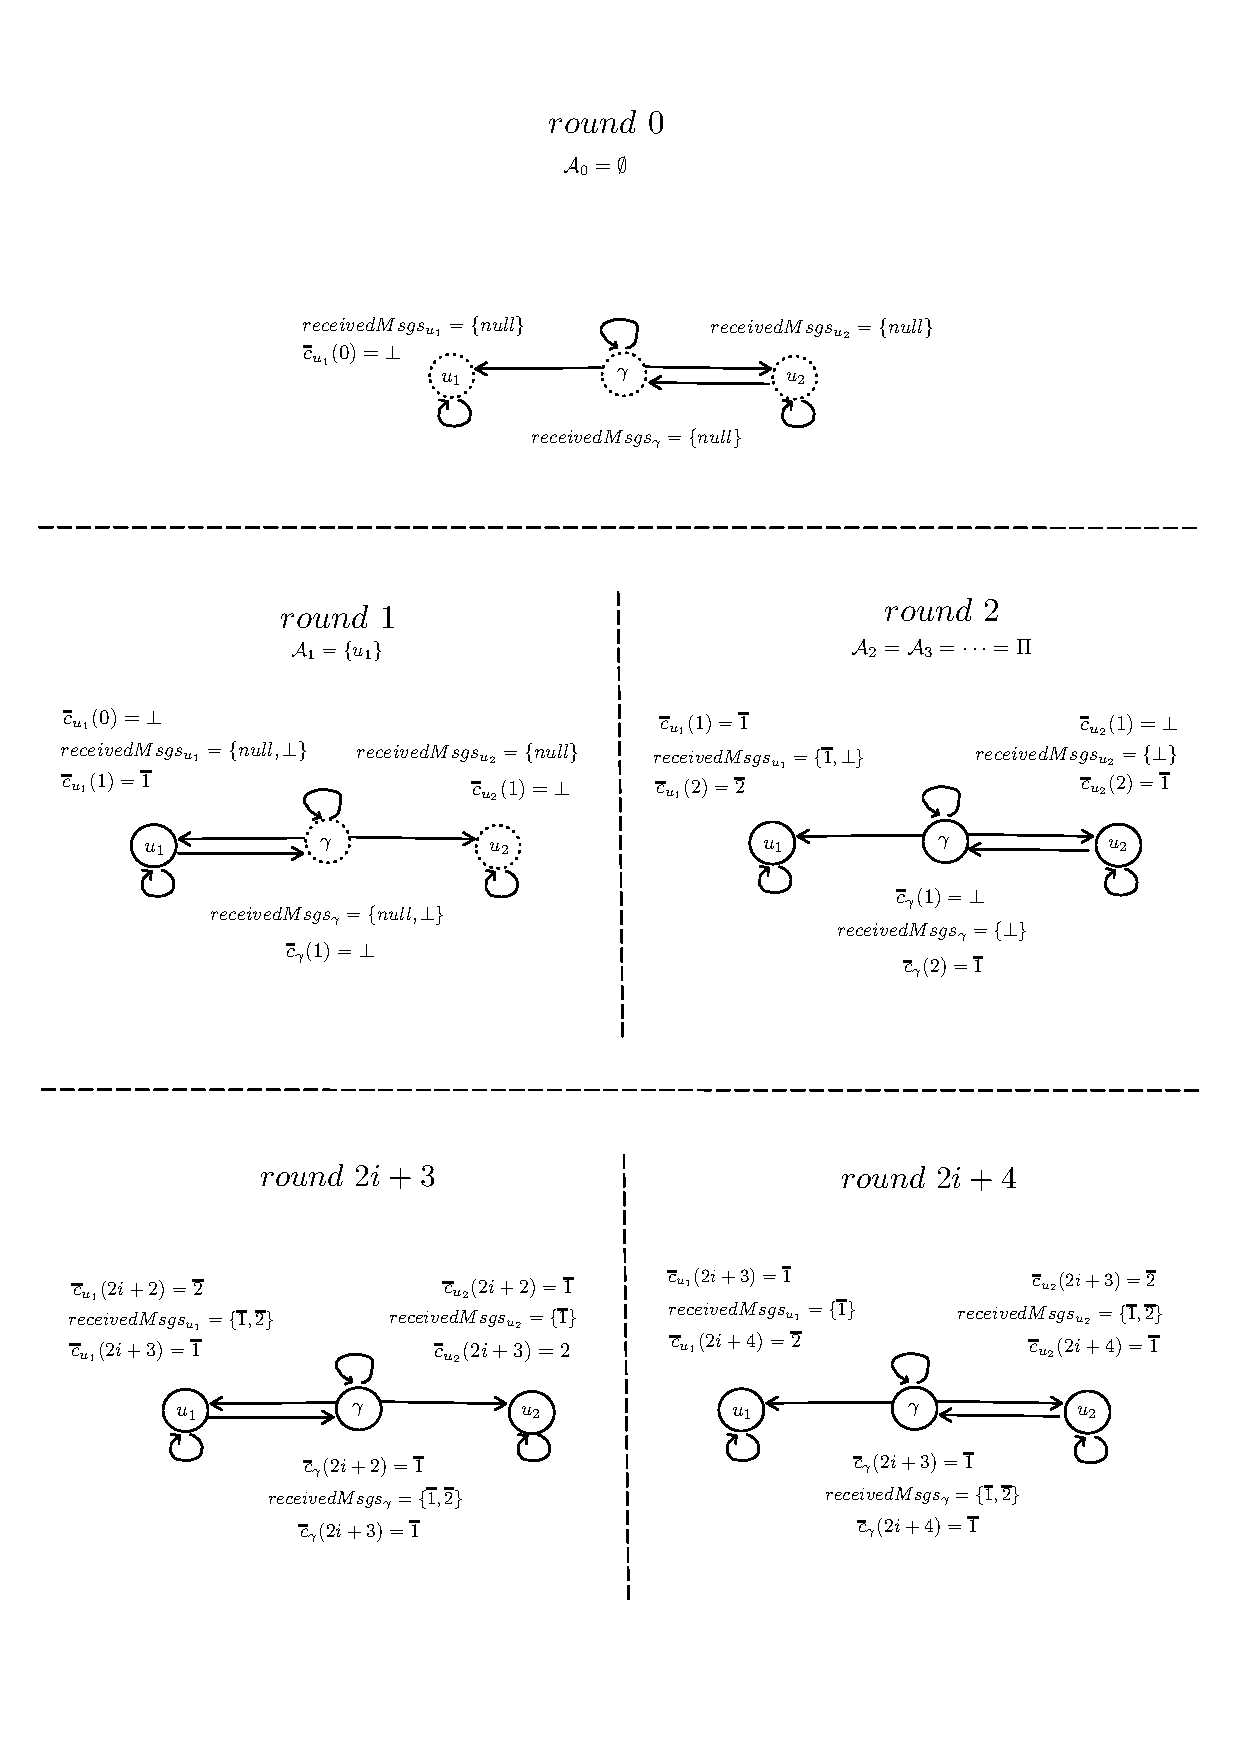
\includepdf[pages=-]{contre_exemple_k_2}



\section{Conclusion and future work}

As any complex reasoning by cases, the correctness proof  of the \SM  algorithm, 
	and more specifically the proof of the liveness property, is very error prone. 
This is a typical example of the relevance and the need of formal verification for distributed algorithms. 
Indeed, in a later work~\cite{}, we used the interactive theorem prover Isabelle to encode the complete proof 
	of Theorem~\ref{thm:k>2}, and thus obtained a certificate for  \SM\!\!'s correctness when $k$ is greater than 2.
	
Since the $\mathrm{mod}\,2$-synchronization is reducible to $\mathrm{mod}\,4$-synchronization,
	 our algorithm solves the $\mathrm{mod}\,k$-synchronization problem for any positive integer~$k$
	 in the class of  dynamic  graphs with a fixed center.
This class of dynamic graphs plays a crucial role regarding benign failures as it captures 
	the general model of at most $n-1$ faulty senders, including the one of at most $n-1$ crashes.
In the widerl context of dynamic graphs, a natural question is whether the problem is still solvable 
	under weaker connectivity assumptions, in particular, in the class of dynamic graphs with a fixed root, 
	i.e., with a time-varying spanning tree at each round rooted at a fixed node.

\printbibliography

\end{document}
